Project launched in October 2014 by Olivier Georgeon on the internet platform MOOC\footnote{\href{http://liris.cnrs.fr/ideal/mooc/}{\texttt{\scriptsize http://liris.cnrs.fr/ideal/mooc/}}\label{noteideal}} consisting of learning and developing a new concept in artificial intelligence called IDEAL (\textbf{I}mplementation of \textbf{DE}velopment\textbf{A}l \textbf{L}earning) -- defined as an ``approach to simulate the early mechanisms of emergent cognition based on theories of enactive cognition and on constructivist epistemology'' \citep{ger}.

\begin{wrapfigure}{r}{0.35\textwidth}
\vspace{-5pt}
   \hspace{-5pt} 
   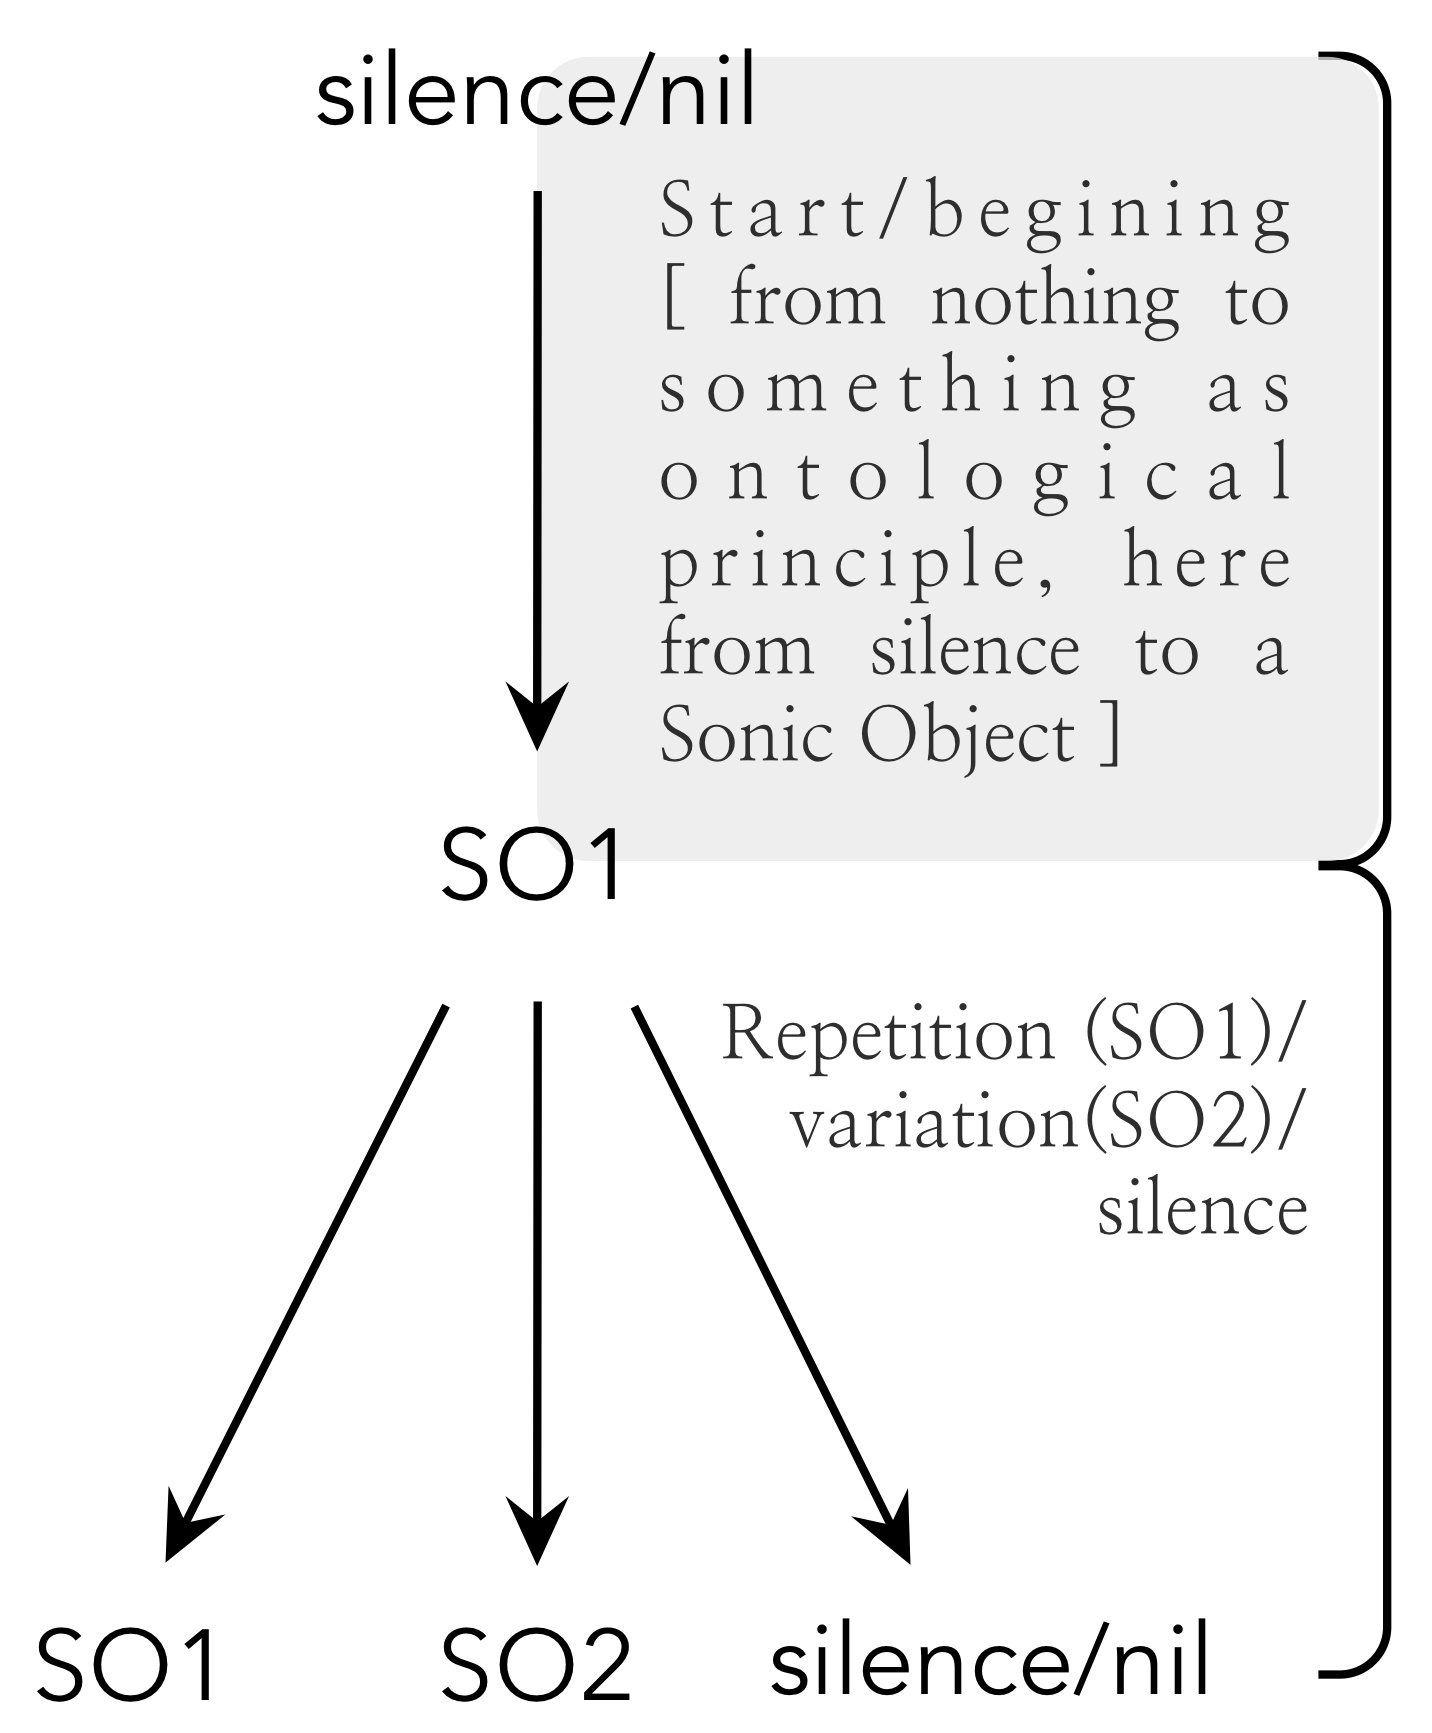
\includegraphics[width=0.35\textwidth]{2345}
  \vspace{-20pt}
\end{wrapfigure}

\bigskip

Then, the idea in the context and in the continuation of \textsl{Neuromuse3}\footnote{\href{https://github.com/yannics/N3D}{\texttt{\scriptsize https://github.com/yannics/N3D}}} is to create a kind of emergent intelligence from the network previously described, composed of cliques and \textit{tournois}, by including additional learning process defined by IDEAL based on the experimentation and on the experience. 

\bigskip

It is opportun to underline the philosophical aspect of this approach in terms of modeling including a causal device as computational cognition.

Thus, each agent develops its own understanding of its environment -- i.e. an ontological conception in epistemological terms.

Also, IDEAL implies non-ontological interactional presuppositions -- the ontological aspect will be defined by the agent as it experiences its interaction with the environment.

\bigskip

With that in mind, the following short description as paragraphs should help the understanding of the different concepts and processes used in this AI context.

\begin{enumerate}[leftmargin=0cm,itemindent=.5cm,labelwidth=\itemindent,labelsep=0cm,align=left]
\item There is \myuline{no a priori knowledge} of the environment. 

\smallskip

`\textit{It allows us to specify inborn behavioral preferences without specifying a predefined goal.}' [$\rightarrow$ \href{https://projet.liris.cnrs.fr/ideal/mooc/lesson.php?n=041}{41. Introduction}, Georgeon, 2014, \textit{loc. cit.} note \ref{noteideal}]

\smallskip

In other words, only primitive interactions -- i.e. innate -- are defined through the initial function, which can evolve over time through the function \texttt{agent-result}. 

\smallskip

`\textit{This design choice follows from constructivist epistemology which suggests that sensorimotor patterns of interaction constitute the basic elements from which the agent constructs knowledge of the world.}' [$\rightarrow$ \href{https://projet.liris.cnrs.fr/ideal/mooc/lesson.php?n=043}{43. Architecture}, Georgeon, 2014, \textit{ibid.}] 

\smallskip

The environment is therefore understood by the AI in terms of reading/writing relevant informations through neurons stimulation device and can be managed by programming constraints.
\end{enumerate}

\bigskip
\bigskip

\noindent {\large \textbf{Glossary}}

\bigskip

Abbreviations: \textsl{fr.} = French; \textsl{acc.} = \textit{acception}.

\begin{description}
\item[Abstract]: is an experiment or a result which refer to an interaction.
\item[Enaction]: interaction with the environment.
\item[Primitive]: low-level interaction defined by the couple experiment/result.\item[Proclivity]: [\textsl{fr}. \textit{propension}] inner, innate, natural force, which directs spontaneously or voluntarily towards an action, a behavior.
\item[Valence]:  [\textsl{acc.} psychology] refers to the intrinsically pleasant or unpleasant quality of a stimulus or situation.
\end{description}

\bigskip

 \begin{notes}

{\large \textbf{Summary description}}

\begin{description}
\item[\texttt{E010}] 
When the expected or desired result is effective, according to the conditions of \texttt{result010}, the qualitative character self-satisfied is `activated' (frustrated otherwise). After $n$ identical, similar, equivalent or other interactions, this is the bored character that is activated, and the system look for another experience to avoid `boredom'.

\item[\texttt{E020}]
The character is quantified with the valence expressing the motivation. This is applied to the primitive interactions.

\quad -- valence $\geq 0 \Rightarrow$ pleased

\quad -- valence $< 0 \Rightarrow$ pained

\item[\texttt{E030}]
Continuation of \texttt{E020} including composite interactions -- i.e. first level abstractions.

\item[\texttt{E031}]
Variation of \texttt{E030} involving weights in terms of proclivity. 

\mynoteuline{The proclivity is estimated as the product of the weight and the} \mynoteuline{valence of the considered interaction.}

\end{description}

\end{notes}

\bigskip

\noindent {\large \textbf{Index}}

\bigskip


\begin{description}[font=\ttfamily]

\item[*PROCLIVITY*] \textit{<t/nil>}

\item[*REMANENCE*] \textit{<integer>}

\item[*VERBOSE*] \textit{<t/nil>}

\item[ADD-OR-GET-EXPERIMENT] \textit{<existence>} \textsl{\&key} label \textit{<symbol>} string \textit{<string>}

\item[ADD-OR-GET-INTERACTION] \textit{<existence>} \textit{<experiment/pre-interaction>} \\ \textit{<result/post-interaction>} \textsl{\&key} valence \textit{<number>} learn \textit{<t/nil>}

\item[ADD-OR-GET-RESULT] \textit{<existence>} \textsl{\&key} label \textit{<symbol>} string \textit{<string>}

\item[CREATE-AGENT] \textit{<name>}

\item[GET-PRIMITIVE-EXPERIENCE] \textit{<experiment/interaction>}

\item[PICK-EXPERIMENT] \textit{<existence>}

\item[PICK-OTHER-EXPERIENCE] \textit{<existence>} \textit{<experiment>}

\item[PREDICT] \textit{<existence>} \textit{<experiment/interaction>} \\ From \textit{existence-interactions}, the evaluation is a \textit{result}.

\item[>REMANENCE] \textit{<existence>} \textit{<experiment/interaction>} \\ Update of \textit{existence-previous} by adding an \textit{experiment} or an \textit{interaction} in the MCT (short-term memory) with |MCT| = \texttt{*REMANENCE*}

\item[RUN-AGENT] <\textit{name}> \textsl{\&key} duration \textit{<integer>} step \textit{<function>} \\ result \textit{<function>}

\item[SELECT-ANTICIPATE] \textit{<existence>} \textit{<experiment/interaction/null>} \\ From \textit{existence-interaction}(s), the evaluation is an \textit{interaction}.

\end{description}






